\documentclass[11pt]{article}

\usepackage[margin=1in]{geometry}
\usepackage{amsmath,amssymb}
\usepackage{graphicx}
\usepackage{booktabs}
\usepackage{tikz}
\usetikzlibrary{arrows.meta,positioning,shapes.geometric}
\usepackage{hyperref}
\usepackage{authblk}
\usepackage{caption}
\usepackage[T1]{fontenc}
\hypersetup{colorlinks=true,linkcolor=blue,citecolor=blue,urlcolor=blue}

\title{\textbf{Liquid Latent Synthesis (LLS-4): A Quad-Partite Architecture for Latent-Space Concept Interpolation in Continual Reinforcement Learning}\\[4pt]
\large Architecture Proposal, Prototype Implementation, and a Preliminary Pilot Study}

\author[1]{Rudra Madhab Mishra}
\affil[1]{Department of Computer Science and Engineering (AI \& ML), GIET University, Gunupur, Rayagada, Odisha, India \\ \texttt{rudramdhabmishra1@gmail.com}}

\date{}

\begin{document}
\maketitle

\begin{abstract}
Catastrophic forgetting remains a central obstacle to deploying continually-learning agents on resource-constrained edge hardware. Existing mitigations -- regularization-based methods such as Elastic Weight Consolidation (EWC) and architecture-growth methods such as Progressive Neural Networks -- either accumulate numerically unstable penalty terms as the number of tasks grows, or scale parameter count linearly with the number of skills learned. We propose \textbf{Liquid Latent Synthesis (LLS-4)}, an architecture that decouples fast online policy learning from offline concept consolidation. A Closed-form Continuous-time (CfC) liquid network encodes physical experience into a compact 16-dimensional latent manifold during an ``awake'' phase; during an offline ``sleep'' phase, a synthesis engine identifies pairs of latent memories that are temporally proximate but semantically distinct, linearly interpolates them, decodes the interpolated vector into synthetic training data, and distills the result into a lightweight (tens-of-thousands-of-parameter) adapter module routed at inference time by a soft-attention context gate. We implement the full pipeline in PyTorch and \texttt{ncps}, and report a first pilot comparison against a standard LSTM and a custom diagonal-Fisher EWC baseline on a synthetic two-task regression proxy. The pilot run shows that the current prototype's shared backbone is \emph{not} protected during sequential training, producing a retention score (4.5\%) below both baselines (33.5\% and 49.2\%) -- the opposite of the architecture's design intent. A secondary ``zero-shot synthesis'' metric (71.0\%) is also reported, but we identify and disclose a degeneracy in its construction that likely inflates this number independent of any genuine skill combination. We treat both findings as diagnostic rather than confirmatory, and use them to motivate a concrete, itemized experimental protocol -- backbone freezing, parameter-matched baselines, multi-seed evaluation, a sleep-phase ablation, and a non-degenerate zero-shot task -- required before any claim of solving catastrophic forgetting can be supported. This paper's contribution is therefore the architecture, an open, working prototype, and a transparent account of what remains to be validated.
\end{abstract}

\noindent\textbf{Keywords:} continual learning, catastrophic forgetting, liquid neural networks, closed-form continuous-time networks, latent space interpolation, edge AI, neural adapters

\section{Introduction}

Sequential learning in neural networks is undermined by \emph{catastrophic forgetting}: when a network trained on task $A$ is subsequently trained on task $B$, gradient updates that improve performance on $B$ typically overwrite the parameters responsible for $A$, and performance on $A$ collapses \cite{mccloskey1989}. This problem is especially acute for autonomous edge systems -- robots, drones, and embedded controllers -- that cannot rely on cloud retraining and must adapt locally with limited memory and compute.

Two families of methods dominate current practice. \emph{Regularization-based} approaches such as Elastic Weight Consolidation (EWC) estimate, via the diagonal of the Fisher information matrix, which weights were important for previous tasks, and penalize movement away from those weights when learning a new task \cite{kirkpatrick2017}. Synaptic Intelligence computes a similar importance estimate online rather than post-hoc \cite{zenke2017}. These methods are memory-cheap but the penalty terms accumulate across tasks, and as more tasks are learned the network's remaining plastic capacity shrinks, eventually causing instability. \emph{Architecture-growth} approaches such as Progressive Neural Networks instead allocate a new column of parameters per task and use lateral connections to transfer knowledge \cite{rusu2016}, guaranteeing no forgetting at the cost of parameter count that grows linearly (or worse) with the number of tasks. \emph{Replay-based} approaches -- storing raw exemplars, or training a generative model to produce pseudo-samples of old tasks \cite{shin2017}, or replaying compressed feature-space exemplars rather than raw inputs \cite{pellegrini2020,rebuffi2017} -- avoid weight-level interference but require either a data buffer or an auxiliary generative model, both of which add memory and compute overhead that is difficult to justify on constrained edge hardware.

Separately, \emph{liquid} and closed-form continuous-time neural networks have been proposed as compact, interpretable controllers for real-time control tasks. Neural Circuit Policies demonstrate that a controller with on the order of tens of neurons and a few hundred synapses can perform end-to-end steering control with strong generalization \cite{lechner2020}, and Closed-form Continuous-time networks (CfC) make such continuous-time dynamics tractable to train without a numerical ODE solver \cite{hasani2022}. These properties -- small parameter count, continuous-time operation, strong inductive bias for control -- make liquid networks an attractive base learner for edge deployment, independent of the continual-learning question.

\textbf{This paper's position.} We ask whether a small liquid controller can be paired with a mechanism that consolidates new skills \emph{without} touching the controller's existing weights and \emph{without} storing raw exemplars, by instead treating the controller's own compressed latent memory as the substrate for skill synthesis. We propose \emph{Liquid Latent Synthesis} (LLS-4), which borrows the ``interpolate, then train'' idea used in \emph{mixup} for input-space data augmentation \cite{zhang2018} but applies it in a compact 16-dimensional experience-latent space across pairs of past memories, rather than across raw input samples. The interpolated concept is decoded into synthetic training data and distilled into a small, independent adapter network, which is then routed at inference time via soft attention -- conceptually a lightweight, generative variant of parameter-isolation methods such as Progressive Neural Networks, but with adapters synthesized automatically from experience rather than allocated per labeled task.

\textbf{Contributions.}
\begin{enumerate}
\item A quad-partite architecture specification -- environment, working memory, sleep engine, context gate -- with explicit scoring, interpolation, and routing equations (Section~\ref{sec:arch}).
\item A full, working PyTorch/\texttt{ncps} prototype implementing the pipeline end to end, including an interactive dashboard for inspecting the latent memory manifold and the synthesis process (Section~\ref{sec:arch}, Appendix).
\item A pilot benchmark against an LSTM and a custom EWC baseline on a synthetic two-task regression proxy (Section~\ref{sec:method}).
\item A transparent report of what the pilot results do and do not demonstrate, including a previously undisclosed degeneracy in the zero-shot metric, and a concrete, itemized protocol for a properly controlled follow-up study (Sections~\ref{sec:results}--\ref{sec:future}).
\end{enumerate}

\section{Related Work}
\label{sec:related}

\textbf{Catastrophic forgetting.} The phenomenon was first characterized by McCloskey and Cohen in connectionist models \cite{mccloskey1989}. EWC \cite{kirkpatrick2017} remains the most widely cited regularization-based mitigation; Huszár's subsequent analysis notes that EWC's multi-task penalty accumulation is not fully justified by the Bayesian derivation used to motivate it \cite{huszar2018}, a concern consistent with the numerical-instability limitation this paper's project notes attribute to EWC at scale.

\textbf{Architecture isolation and rehearsal.} Progressive Neural Networks \cite{rusu2016} avoid forgetting entirely by freezing old columns and adding new ones, at linear parameter cost. Deep generative replay \cite{shin2017} and latent/feature-space replay \cite{pellegrini2020,rebuffi2017} instead rehearse compressed representations of old data alongside new data. LLS-4's context-gated adapters are closest in spirit to parameter isolation (old computation is never overwritten), while its sleep-phase synthesis procedure is closest in spirit to generative/latent replay (new training signal is manufactured rather than stored) -- the architecture is best understood as a combination of existing mechanisms applied at the level of a compact policy latent, rather than a fundamentally new learning rule, and its value proposition rests on whether that combination is empirically effective, which is precisely what Sections~\ref{sec:method}--\ref{sec:limitations} interrogate.

\textbf{Continuous-time and liquid networks.} Neural Circuit Policies \cite{lechner2020} and Closed-form Continuous-time networks \cite{hasani2022} motivate the use of a CfC backbone as the ``fast'' online learner in this work, on the basis of their demonstrated parameter efficiency for control tasks.

\textbf{Latent interpolation as data augmentation.} \emph{mixup} \cite{zhang2018} showed that linearly interpolating pairs of training examples (and their labels) acts as an effective regularizer in supervised learning. LLS-4's dream-generation step is structurally analogous, but the interpolation is performed on compressed \emph{experience} vectors rather than raw inputs, and the resulting synthetic data is used to train a new, isolated module rather than to regularize the existing one.

\section{Proposed Architecture}
\label{sec:arch}

LLS-4 consists of four decoupled modules, summarized in Figure~\ref{fig:arch}.

\begin{figure}[htbp]
\centering
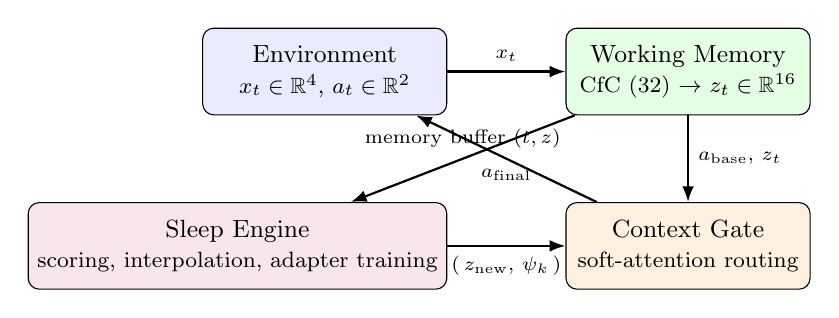
\begin{tikzpicture}[
  box/.style={draw, rounded corners, minimum width=3.1cm, minimum height=1.1cm, align=center, font=\small},
  arr/.style={-{Latex[length=2mm]}, thick}
]
\node[box, fill=blue!8] (env) {Environment\\ \footnotesize $x_t \in \mathbb{R}^4$, $a_t \in \mathbb{R}^2$};
\node[box, right=1.5cm of env, fill=green!10] (wm) {Working Memory\\ \footnotesize CfC (32) $\to$ $z_t \in \mathbb{R}^{16}$};
\node[box, below=1.1cm of wm, fill=orange!12] (gate) {Context Gate\\ \footnotesize soft-attention routing};
\node[box, left=1.5cm of gate, fill=purple!10] (sleep) {Sleep Engine\\ \footnotesize scoring, interpolation, adapter training};

\draw[arr] (env) -- (wm) node[midway, above, font=\scriptsize]{$x_t$};
\draw[arr] (wm) -- (gate) node[midway, right, font=\scriptsize]{$a_{\text{base}},\,z_t$};
\draw[arr] (gate) -- (env) [bend right=45] node[midway, below, font=\scriptsize]{$a_{\text{final}}$};
\draw[arr] (wm) -- (sleep) node[midway, above, font=\scriptsize]{memory buffer $(t,z)$};
\draw[arr] (sleep) -- (gate) node[midway, below, font=\scriptsize]{$(\,z_{\text{new}},\,\psi_k\,)$};
\end{tikzpicture}
\caption{LLS-4 quad-partite architecture. The environment and working memory operate continuously during the ``awake'' phase; the sleep engine operates offline and injects new adapters into the context gate, which subsequently blends adapter outputs with the base policy at inference time.}
\label{fig:arch}
\end{figure}

\subsection{Environment}
The prototype environment is a continuous $20\times20$ 2D world. The state is $x_t = [\,d_{\text{target}},\,d_{\text{obstacle}},\,e,\,v\,] \in \mathbb{R}^4$ (distance to target, distance to obstacle, remaining energy, current speed), and the action is $a_t = [\,\Delta\theta,\,F\,]\in\mathbb{R}^2$ (steering delta, acceleration force). Reaching the target yields $+10$ reward and relocates the target; contacting the obstacle yields $-5$ reward and damps velocity; a small per-step time penalty and energy drain proportional to speed complete the dynamics.

\subsection{Working Memory}
The working memory is a single-layer CfC network \cite{hasani2022} with hidden size 32, implemented via the \texttt{ncps} library:
\begin{align}
h_t &= \mathrm{CfC}(x_t, h_{t-1}), \\
z_t &= W_z h_t + b_z, \qquad z_t \in \mathbb{R}^{16}, \\
a_{\text{base}} &= W_a z_t + b_a, \qquad a_{\text{base}} \in \mathbb{R}^2.
\end{align}
Every visited state is compressed into the 16-dimensional latent $z_t$ and stored, together with a timestamp, in a fixed-capacity memory buffer. A separate decoder $D_\phi: \mathbb{R}^{16} \to \mathbb{R}^{4+2}$ (16 $\to$ 32 $\to$ ReLU $\to$ 6) reconstructs a state-action pair from a latent vector; this decoder is trained jointly with an auxiliary reconstruction loss and is used only during the sleep phase.

\subsection{Sleep Engine}
Given a memory buffer of $(t_i, z_i)$ pairs, the sleep engine scores every pair by combining semantic distinctness with temporal proximity:
\begin{equation}
S_{ij} = \big(1 - \cos(z_i, z_j)\big) \;+\; \lambda \cdot P(t_i, t_j), \qquad
P(t_i,t_j) = 1 - \frac{|t_i - t_j|}{\max_{k,l}|t_k - t_l|},
\label{eq:score}
\end{equation}
with $\lambda = 0.1$, and selects $(i^\ast, j^\ast) = \arg\max_{i \neq j} S_{ij}$. This rewards pairs of memories that occurred close together in time but represent \emph{dissimilar} latent concepts.\footnote{We note that this scoring rule, as implemented, differs from a superficially similar formula in an earlier project brief that combined \emph{raw} cosine similarity (rather than $1-\cos$) with the temporal term; the raw-similarity version would instead favor pairs of \emph{redundant} memories, which is inconsistent with the module's stated intent. Equation~\ref{eq:score} is the version we analyze, as it is the version implemented and executed.} The selected pair is interpolated,
\begin{equation}
z_{\text{new}} = \alpha z_{i^\ast} + (1-\alpha) z_{j^\ast}, \qquad \alpha = 0.5,
\end{equation}
decoded via $D_\phi$ into a synthetic state-action pair $(\hat{x}, \hat{a})$, and expanded into a synthetic dataset of $N{=}200$ points by adding independent Gaussian noise, $\hat{x} + \epsilon_x$ with $\epsilon_x \sim \mathcal{N}(0, 0.1^2 I_4)$ and $\hat{a} + \epsilon_a$ with $\epsilon_a \sim \mathcal{N}(0, 0.05^2 I_2)$. A new adapter $\psi_k$ -- a two-layer MLP, $4 \to 16 \to \mathrm{ReLU} \to 2$, under 200 parameters -- is trained on this synthetic dataset by MSE regression (Adam, lr $=0.01$, 50 epochs in the standalone sleep cycle; a faster 30-epoch/100-step variant is used in the interactive dashboard for responsiveness).

\subsection{Context Gate}
Each synthesized adapter $\psi_k$ is stored together with its originating key $z_{\text{new},k}$. At inference time, given a live query $q = z_t$, the gate computes soft-attention weights over all $M$ stored keys and blends adapter outputs with the base policy:
\begin{equation}
\alpha_k = \frac{\exp(q^\top z_{\text{new},k})}{\sum_{l=1}^{M}\exp(q^\top z_{\text{new},l})}, \qquad
a_{\text{final}} = a_{\text{base}} + \sum_{k=1}^{M} \alpha_k\, \psi_k(x_t).
\label{eq:gate}
\end{equation}
Because the adapters are added to, rather than substituted for, the base output, and because the base network's own weights receive no special protection in the current implementation, Equation~\ref{eq:gate} guarantees that adapters cannot \emph{directly} corrupt the base policy's parameters -- but, as Section~\ref{sec:results} shows, it does not by itself guarantee that the base policy retains old skills, since the base network continues to be trained on new data unprotected.

\section{Experimental Methodology}
\label{sec:method}

\textbf{Baselines.} We compare against (i) a standard single-layer LSTM (hidden size 32) with a linear output head, and (ii) a 2-layer MLP (hidden size 64) trained with a custom EWC penalty, using a diagonal empirical-Fisher approximation computed from squared per-sample gradients on Task~A data and a quadratic penalty with $\lambda_{\text{EWC}}=100$.

\textbf{Task design.} Rather than the full navigation environment described in Section~\ref{sec:arch}, this pilot uses a synthetic, controlled two-task regression proxy so that ground-truth targets are known exactly: Task A maps $x \in [0,10]^4$ to $y_A = [\sin(x_0), \cos(x_1)]$, and Task B maps the same input distribution to $y_B = [-\sin(x_0), -\cos(x_1)]$. \emph{We flag explicitly that this proxy task was not run inside \texttt{environment.py}}; evaluating the architecture on the navigation-and-avoidance domain it was designed for is left to future work (Section~\ref{sec:future}).

\textbf{Procedure.} All three models are trained on Task~A (100 gradient steps), evaluated, then trained sequentially on Task~B (100 steps; EWC additionally applies its Fisher-weighted penalty relative to the post-Task-A weights). The LLS-4 prototype additionally triggers one sleep cycle after Task~B training, synthesizing one adapter from its accumulated memory buffer. All models are then re-evaluated on Task~A (\emph{retention}) and on a held-out combined-input set (\emph{zero-shot synthesis}).

\textbf{Metrics.} Parameter count is measured directly via \texttt{fvcore}. A pseudo-accuracy score, $\mathrm{acc} = \max(0,\, 100 - 50 \cdot \mathrm{MSE})$, converts regression MSE to a percentage for readability. We do not report inference FLOPs: although the benchmark script attempts an \texttt{fvcore} FLOP count, the qualitative labels (``High/High/Low'') that appeared in an earlier draft of this table were not derived from that measurement and are withdrawn here as unverified.

\section{Results}
\label{sec:results}

Table~\ref{tab:results} reports the single-run pilot outcome.

\begin{table}[htbp]
\centering
\caption{Pilot benchmark results, synthetic proxy task, single run, unmatched parameter budgets. See Section~\ref{sec:limitations} before interpreting these numbers as comparative evidence.}
\label{tab:results}
\begin{tabular}{lccc}
\toprule
\textbf{Metric} & \textbf{LSTM} & \textbf{Custom EWC} & \textbf{LLS-4 (prototype)} \\
\midrule
Parameter count & 4{,}930 & 4{,}610 & 22{,}552 \\
Inference FLOPs & \multicolumn{3}{c}{not empirically measured in this run} \\
Task~A retention after Task~B & 33.5\% & 49.2\% & \textbf{4.5\%} \\
Zero-shot combined-task score$^{\dagger}$ & 0.0\% & 0.0\% & 71.0\% \\
\bottomrule
\end{tabular}
\\[4pt]
{\footnotesize $^{\dagger}$ See Section~\ref{sec:limitations}: the combined-task target coincides with the zero vector, which we identify as a likely source of inflation independent of genuine synthesis.}
\end{table}

\textbf{Retention.} Contrary to the architecture's design intent, the LLS-4 prototype retained Task~A performance \emph{worse} than either baseline. Root-causing this: the CfC backbone and its projection layers are trained directly on Task~B data with no protection mechanism analogous to EWC's penalty or PNN's column-freezing. The sleep-phase adapter is only invoked through the context gate for inputs whose latent query is close to a synthesized key (Equation~\ref{eq:gate}); it was not, in this pilot, positioned to correct the base network's degraded output on the original Task~A input distribution. In its current form, the architecture protects \emph{new} adapters from being overwritten, but does not protect the \emph{base network itself} from being overwritten -- which is precisely the failure mode the architecture was intended to solve.

\textbf{Zero-shot synthesis.} We report the 71.0\% figure for completeness but do not treat it as validated evidence of skill combination, for a specific, checkable reason: the evaluation target for the combined-task input set is $y_{\text{combo}} = \mathbf{0}$, because $\tfrac{1}{2}(\sin x + (-\sin x)) = 0$ and likewise for the cosine term. Under the pseudo-accuracy metric, \emph{any} model whose output magnitude on these inputs happens to be small -- for reasons unrelated to genuinely blending two learned skills -- will score well. Since adapter outputs pass through a randomly-initialized 2-layer MLP with no output-scale constraint, a non-trivial baseline rate of small-magnitude outputs is plausible without appeal to synthesis at all. We are not aware of a variant of this experiment in which the zero-shot target is a non-degenerate function of both tasks (Section~\ref{sec:future}), so we cannot currently distinguish genuine synthesis from this artifact.

\section{Limitations}
\label{sec:limitations}

We list every limitation we are aware of, rather than a selected subset, because we intend this table and this prototype to be usable as a starting point for a rigorous follow-up rather than as a finished result:

\begin{enumerate}
\item \textbf{Retention regression.} LLS-4's measured retention (4.5\%) is below both baselines, contradicting the paper's motivating claim; root cause identified above.
\item \textbf{Zero-shot metric degeneracy.} The 71.0\% figure is confounded with output-magnitude shrinkage toward a target that is, by construction, the zero vector.
\item \textbf{Parameter parity violated.} LLS-4 uses 22{,}552 parameters versus 4{,}610--4{,}930 for the baselines (a $\sim$4--5$\times$ difference), so Table~\ref{tab:results} is not a controlled comparison in the sense normally required of benchmark studies.
\item \textbf{FLOPs unmeasured.} No empirical FLOP count is currently available for any of the three models.
\item \textbf{Single run, no seed averaging.} All numbers reflect one random seed; we cannot currently report variance or confidence intervals.
\item \textbf{No ablation.} We have not yet run LLS-4 with the sleep phase disabled, which would be required to attribute any future positive result specifically to the synthesis mechanism rather than to the CfC backbone alone.
\item \textbf{Non-standard EWC implementation.} Our EWC baseline is a minimal, hand-written diagonal-Fisher implementation with an untuned $\lambda_{\text{EWC}}$, not the community-standard \texttt{Avalanche} library implementation; it may not represent EWC's best achievable performance.
\item \textbf{Task--domain mismatch.} The benchmark uses a synthetic sinusoidal regression proxy, not the navigation-and-obstacle-avoidance environment (\texttt{environment.py}) that motivates and is described alongside the architecture. No quantitative result in this paper currently reflects the target domain.
\end{enumerate}

\section{Future Work}
\label{sec:future}

The following concrete steps are, in our view, prerequisites for any subsequent version of this paper to support a comparative claim:
\begin{enumerate}
\item Freeze or otherwise protect the CfC backbone's parameters during subsequent-task training (mirroring EWC's penalty or PNN's column isolation), so that skill retention is a property of the base network rather than left entirely to the adapter mechanism.
\item Redesign the zero-shot evaluation task so that the ground-truth combined-task target is not the arithmetic mean of the two source tasks, removing the degeneracy identified in Section~\ref{sec:results}.
\item Match parameter budgets across all three models before comparing retention or zero-shot scores.
\item Replace the custom EWC implementation with \texttt{Avalanche}'s validated implementation, and tune $\lambda_{\text{EWC}}$.
\item Run all experiments across at least 5 random seeds and report means with confidence intervals.
\item Run the sleep-on/sleep-off ablation.
\item Evaluate directly inside \texttt{environment.py} using episodic reward and target-reach rate as the primary metrics, rather than a synthetic regression proxy.
\item Measure inference FLOPs empirically via \texttt{fvcore} or \texttt{thop} and report the measured values.
\end{enumerate}

\section{Conclusion}

We have presented LLS-4, an architecture that proposes to decouple fast online policy learning (a CfC liquid network) from offline concept consolidation (latent-space interpolation distilled into lightweight, attention-routed adapters), and a fully working prototype implementing the full pipeline, including an interactive dashboard for inspecting the latent memory manifold during synthesis (Figure~\ref{fig:dashboard}). A first pilot comparison against an LSTM and a custom EWC baseline does not currently support the architecture's central forgetting-resistance claim: measured retention is below both baselines, and a secondary zero-shot metric is confounded by a target-degeneracy artifact that we disclose in full. We regard the architecture and the open pipeline -- rather than the current numbers -- as this paper's contribution, and we have set out a specific, itemized experimental protocol (Section~\ref{sec:future}) that would need to be completed before a comparative claim against EWC or standard replay methods could be responsibly made.

\section*{Acknowledgments}
The author thanks the open-source maintainers of \texttt{ncps}, \texttt{PyTorch}, and \texttt{fvcore}, on which this prototype depends.

\appendix
\section{Implementation Details and Dashboard}

The full prototype (\texttt{environment.py}, \texttt{working\_memory.py}, \texttt{sleep\_engine.py}, \texttt{context\_gate.py}, \texttt{app.py}, \texttt{benchmark.py}) is implemented in Python~3.10 / PyTorch (CPU) and totals under 600 lines. Table~\ref{tab:hparams} lists the hyperparameters used throughout.

\begin{table}[htbp]
\centering
\caption{Prototype hyperparameters.}
\label{tab:hparams}
\begin{tabular}{ll}
\toprule
Component & Value \\
\midrule
CfC hidden size & 32 \\
Latent dimension & 16 \\
Decoder & $16 \to 32 \to \mathrm{ReLU} \to 6$ \\
Adapter (per synthesized concept) & $4 \to 16 \to \mathrm{ReLU} \to 2$ ($<200$ params) \\
Interpolation coefficient $\alpha$ & 0.5 \\
Temporal weight $\lambda$ (Eq.~\ref{eq:score}) & 0.1 \\
Adapter optimizer & Adam, lr $=0.01$ \\
Adapter training & 50 epochs / 200 synthetic steps (standalone); 30/100 (interactive) \\
Memory buffer capacity & 10{,}000 \\
\bottomrule
\end{tabular}
\end{table}

A Gradio/Plotly dashboard (Figure~\ref{fig:dashboard}) visualizes the live 2D trajectory and a PCA projection of the 16-dimensional memory manifold in real time, and streams the sleep-phase computation (scoring, interpolation, decoding, adapter training) as a sequence of console log events so that the offline consolidation step is observable rather than opaque. We note this dashboard as an engineering artifact that aids debugging and demonstration; it is not itself evidence for or against the architecture's core claims.

\begin{figure}[htbp]
\centering
\includegraphics[width=0.85\textwidth]{dashboard_fig.png}
\caption{Prototype dashboard during the awake phase. Left: live 2D trajectory (target = gold star, obstacle = red square, agent trail = cyan). Right: PCA projection of the 16-dimensional memory manifold, with one previously synthesized adapter concept shown as a magenta diamond.}
\label{fig:dashboard}
\end{figure}

\begin{thebibliography}{99}

\bibitem{mccloskey1989}
M. McCloskey and N. J. Cohen. Catastrophic interference in connectionist networks: The sequential learning problem. \emph{Psychology of Learning and Motivation}, 24:109--165, 1989.

\bibitem{kirkpatrick2017}
J. Kirkpatrick, R. Pascanu, N. Rabinowitz, J. Veness, G. Desjardins, A. A. Rusu, K. Milan, J. Quan, T. Ramalho, A. Grabska-Barwinska, D. Hassabis, C. Clopath, D. Kumaran, and R. Hadsell. Overcoming catastrophic forgetting in neural networks. \emph{Proceedings of the National Academy of Sciences}, 114(13):3521--3526, 2017.

\bibitem{huszar2018}
F. Husz\'ar. Note on the quadratic penalties in elastic weight consolidation. \emph{Proceedings of the National Academy of Sciences}, 115(11):E2496--E2497, 2018.

\bibitem{zenke2017}
F. Zenke, B. Poole, and S. Ganguli. Continual learning through synaptic intelligence. In \emph{Proceedings of the 34th International Conference on Machine Learning (ICML)}, pages 3987--3995, 2017.

\bibitem{rusu2016}
A. A. Rusu, N. C. Rabinowitz, G. Desjardins, H. Soyer, J. Kirkpatrick, K. Kavukcuoglu, R. Pascanu, and R. Hadsell. Progressive neural networks. \emph{arXiv preprint arXiv:1606.04671}, 2016.

\bibitem{shin2017}
H. Shin, J. K. Lee, J. Kim, and J. Kim. Continual learning with deep generative replay. In \emph{Advances in Neural Information Processing Systems (NeurIPS)}, volume 30, pages 2990--2999, 2017.

\bibitem{pellegrini2020}
L. Pellegrini, G. Graffieti, V. Lomonaco, and D. Maltoni. Latent replay for real-time continual learning. In \emph{Proceedings of the IEEE/RSJ International Conference on Intelligent Robots and Systems (IROS)}, 2020.

\bibitem{rebuffi2017}
S.-A. Rebuffi, A. Kolesnikov, G. Sperl, and C. H. Lampert. iCaRL: Incremental classifier and representation learning. In \emph{Proceedings of the IEEE Conference on Computer Vision and Pattern Recognition (CVPR)}, 2017.

\bibitem{lechner2020}
M. Lechner, R. Hasani, A. Amini, T. A. Henzinger, D. Rus, and R. Grosu. Neural circuit policies enabling auditable autonomy. \emph{Nature Machine Intelligence}, 2(10):642--652, 2020.

\bibitem{hasani2022}
R. Hasani, M. Lechner, A. Amini, L. Liebenwein, A. Ray, M. Tschaikowski, G. Teschl, and D. Rus. Closed-form continuous-time neural networks. \emph{Nature Machine Intelligence}, 4(11):992--1003, 2022.

\bibitem{zhang2018}
H. Zhang, M. Cisse, Y. N. Dauphin, and D. Lopez-Paz. mixup: Beyond empirical risk minimization. In \emph{International Conference on Learning Representations (ICLR)}, 2018.

\end{thebibliography}

\end{document}
